\documentclass[adobefonts, nocap]{ctexart}
\usepackage{amsmath}
% \usepackage{amsfonts}
\usepackage{tikz}
\usepackage{tikz-qtree}
\usepackage{caption}
\usepackage{hyperref}
\hypersetup{
  colorlinks = true,
  linkcolor = blue,
  unicode = true
}
\captionsetup{belowskip = 12pt, aboveskip = 10pt}
\tikzset{every tree node/.style = {align = center, anchor = north}}
\begin{document}
  \title{计算机系统结构第二次作业}
  \author{李雨田\hspace{1em}2010012193\hspace{1em}计14}
  \maketitle
  \section*{2.11}
    不难构造如下Huffman树,
    \begin{figure}[h]
      \centering
      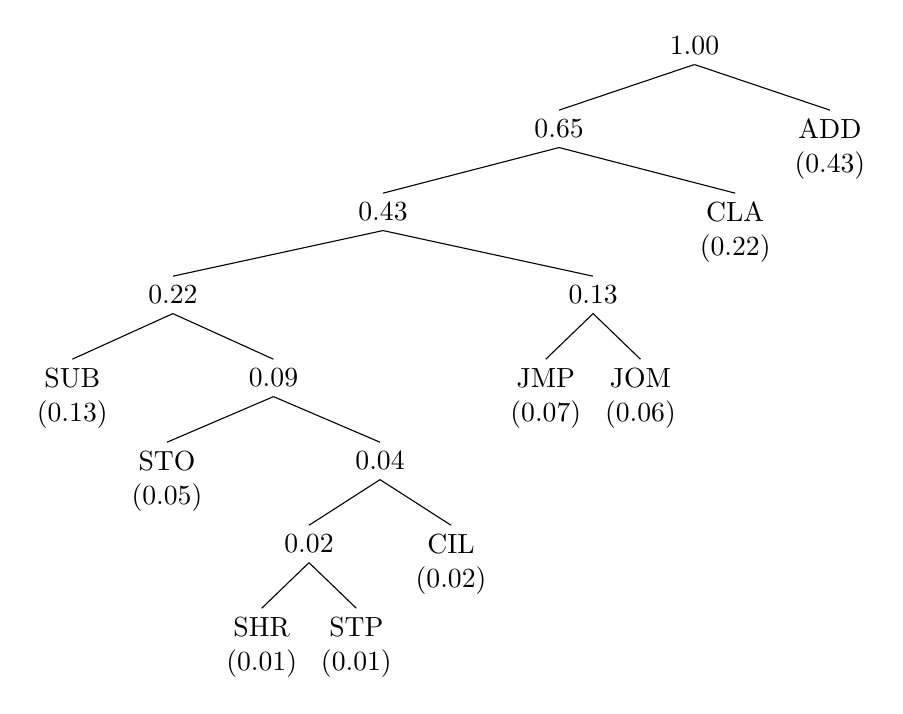
\begin{tikzpicture}
        \Tree [.1.00 [.0.65 [.0.43 [.0.22 {SUB \\ (0.13)} [.0.09 {STO \\ (0.05)} [.0.04 [.0.02 {SHR \\ (0.01)} {STP \\ (0.01)} ] {CIL \\ (0.02)} ] ] ] [.0.13 {JMP \\ (0.07)} {JOM \\ (0.06)} ] ] {CLA \\ (0.22)} ] {ADD \\ (0.43)} ]
      \end{tikzpicture}
    \end{figure}

    定义向左为$0$,向右为$1$.可以得到一个Huffman编码.对于3/3/3扩展编码,位数分别是2, 4, 6位.对于2/7扩展编码,位数分别是2, 4位.按频率得到表\ref{t1}.
    \begin{table}[h]
      \centering
      \caption{编码}
      \label{t1}
      \begin{tabular}{c||c|c|c}
        Instruction & Huffman Encoding & 3/3/3 Encoding & 2/7 Encoding \\
        \hline
        \hline
        ADD & 1 & 00 & 00 \\
        \hline
        CLA & 01 & 01 & 01 \\
        \hline
        SUB & 0000 & 10 & 1000 \\
        \hline
        JMP & 0010 & 1100 & 1001 \\
        \hline
        JOM & 0011 & 1101 & 1010 \\
        \hline
        STO & 00010 & 1110 & 1011 \\
        \hline
        CIL & 000111 & 111100 & 1100 \\
        \hline
        SHR & 0001100 & 111101 & 1101 \\
        \hline
        STP & 0001101 & 111110 & 1110 \\
      \end{tabular}.
    \end{table}

    根据$\sum p_{i}I_{i}$计算三者的平均码长.Huffman编码的平均码长是$2.42$, 3/3/3扩展编码的平均码长是$2.52$, 2/7扩展编码的平均码长是$2.70$.
  \section*{2.12}
    单地址指令为$10$位操作码和$6$位地址码,两地址指令为$4$位操作码和$12$位操作码.若两地址指令有$A$条,在编码中占$2^{12}A$条编码,剩下$2^{16}-2^{12}A$条编码.一条单地址指令需要$2^{6}$条编码,则单地址指令最多有
    \[
      \frac{2^{16}-2^{12}A}{2^{6}}=2^{10}-2^{6}A.
    \]
  \section*{2.13}
    先从三地址指令开始编码,地址码占$9$位,留给操作码的只有$3$位.操作码共有$4$条,占了$2$位,还留下$1$位用来扩展,此时可分配的操作码至多只有$11$位,共$2^{11}$条.单地址指令地址码占$3$位,留给操作码的只有$8$位.单地址指令共有$255=2^{8}-1$条,留下$1$条用来扩展.但此时操作码只有$3$位,至多编码$8$条指令,而零地址指令有$16$条,所以不能用扩展编码为其操作码编码.

    如果单地址指令为$254$条,则单地址指令编码后可剩下$2$条指令扩展,共有$2\times 2^{3}=16$,足够为零地址指令编码.可以使用扩展编码为其操作码编码.
\end{document}
